\documentclass{article}

% if you need to pass options to natbib, use, e.g.:
%\PassOptionsToPackage{authoryear, square}{natbib}
%\PassOptionsToPackage{numbers, authoryear, square}{natbib}
% before loading nips_2017
%
% to avoid loading the natbib package, add option nonatbib:
%\usepackage[nonatbib]{ner}

\usepackage[final]{ner}

% to compile a camera-ready version, add the [final] option, e.g.:
% \usepackage[final]{nips_2017}

\usepackage[utf8]{inputenc} % allow utf-8 input
\usepackage[T1]{fontenc}    % use 8-bit T1 fonts
\usepackage{hyperref}       % hyperlinks
\usepackage{url}            % simple URL typesetting
\usepackage{booktabs}       % professional-quality tables
\usepackage{amsfonts}       % blackboard math symbols
\usepackage{nicefrac}       % compact symbols for 1/2, etc.
\usepackage{microtype}      % microtypography
\usepackage{subcaption}
\usepackage{amsmath}

\usepackage[pdftex]{graphicx}
\usepackage{fancyhdr}
\usepackage[subpreambles=true]{standalone} 
\usepackage{tikz}

\usepackage{array}
\usepackage{amsfonts}
\usepackage{mathbbol}
\usepackage[ruled]{algorithm}
\usepackage{algpseudocode}

%% abbreviations
\newcommand{\ie}{\textit{i.e.}}
\newcommand{\st}{\textit{s.t.}}
\newcommand{\eg}{\textit{e.g.}}
\newcommand{\etc}{\textit{etc}}
\newcommand{\etal}{\textit{et~al.}}
\newcommand{\tuple}[1]{\ensuremath{( #1 )}\xspace}


\title{\nrc: a decentralized platform for Human-Robot Communication}

% The \author macro works with any number of authors. There are two
% commands used to separate the names and addresses of multiple
% authors: \And and \AND.
%
% Using \And between authors leaves it to LaTeX to determine where to
% break the lines. Using \AND forces a line break at that point. So,
% if LaTeX puts 3 of 4 authors names on the first line, and the last
% on the second line, try using \AND instead of \And before the third
% author name.

% An example of author info
%Chen Min\thanks{Use footnote for providing further
%information about author (webpage, alternative
%address)---\emph{not} for acknowledging funding agencies.} \\
%Department of Computer Science\\
%NUS, Singapore\\
%\texttt{chenmin@comp.nus.edu.sg} \\

\author{
  Chen Min, PhD\thanks{Expected to graduate in Aug 2018}\\
  NEO Robotics
  \\
  NUS, Singapore\\
  \texttt{chenmin@comp.nus.edu.sg} \\
  \And
  Xie Shudong, PhD\thanks{Expected to graduate in Dec 2017}\\
  NEO Robotics
  \thanks{NEO Robotics is the name of our team.
      The objective of our team is to use blockchain technology
      to improve robots' capabilities and safety when working 
      with humans.}
  \\
  Singapore\\
  \texttt{purplebamboot@gmail.com} \\
  \And
  Chen Liyuan, Msc\\
  NEO Robotics\\
  Singapore\\
  \texttt{colacly@gmail.com} \\
  %% examples of more authors
  %% \And
  %% Coauthor \\
  %% Affiliation \\
  %% Address \\
  %% \texttt{email} \\
  %% \AND
  %% Coauthor \\
  %% Affiliation \\
  %% Address \\
  %% \texttt{email} \\
  %% \And
  %% Coauthor \\
  %% Affiliation \\
  %% Address \\
  %% \texttt{email} \\
  %% \And
  %% Coauthor \\
  %% Affiliation \\
  %% Address \\
  %% \texttt{email} \\
}

\begin{document}
% \nipsfinalcopy is no longer used

\maketitle

\begin{abstract}
	
More and more robots are coming into human's daily life,
\eg, autonomous driving car and household robot.
Unlike traditional robots in the factory, robots that share the
same workspace with humans have to (i) gather information on humans'
physical state and mental state;
and (ii) take actions to achieve their own objectives.
Currently, most robots rely purely on onboard sensors to gather 
information, such as lidar and camera.
However, those sensors might fail due to weather or lighting
conditions, which might result in fatal accidents.
% topic
This paper introduces NRC, 
a decentralized platform built on NEO blockchain
for trust-free human-robot communication.
With \nrc, the human and the robot are able to broadcast their
information on the blockchain, and receive the 
information from other agents for their decision making.
% the adavantage of NER, and the impact
% 1. compared with onboard sensors
Compared with onboard sensors, NRC can provides additional 
information for the robot that can not be achieved by 
any sensors available.
For example, with \nrc, the robot will be able to know the 
intention of humans.
% 2. compared with the traditional communication device
Compared to the traditional communication protocols, 
the blockchain based
NRC provides serveral adavantages:
(i) it reduces the cost of trust, \ie, the human and the robot can trust
the information they received is correct. This is handled automatically
by the smart contracts without any extra effort.
(ii) the NRC token gives incentive for the human to share
their information to the robots, \ie, the human gets paid instantly
when his/her information is used by a robot.
As a proof of concept, we test NRC in the scenario of autonomous driving,
where we demonstrate the adavantages that NRC provides.
Note that NRC is general and not limit to autonomous driving. 
It can
be potentially applied on any robots that share their workspace
with humans.
 
\end{abstract}


\section{Introduction}

% Motivation
In the past decades, dramatic prograss has been made in the field
of robotics~\cref{thrun2005probabilistic,siciliano2016springer}.
Robots are moving from factories, where robots have their own workspace,
into people's daily life, where robots share their workspace with 
humans (\figref{fig:robots}).
% Examples
There is an urgent need for developing robotic systems that can work closely with
human without hurting human or disturbing human's working 
flow~\cref{goodrich2007human,broz2008planning}.

\begin{figure}[t!]
    \centering
    \begin{tabular}{rr}
        \begin{subfigure}{0.99\linewidth}
            \centering
            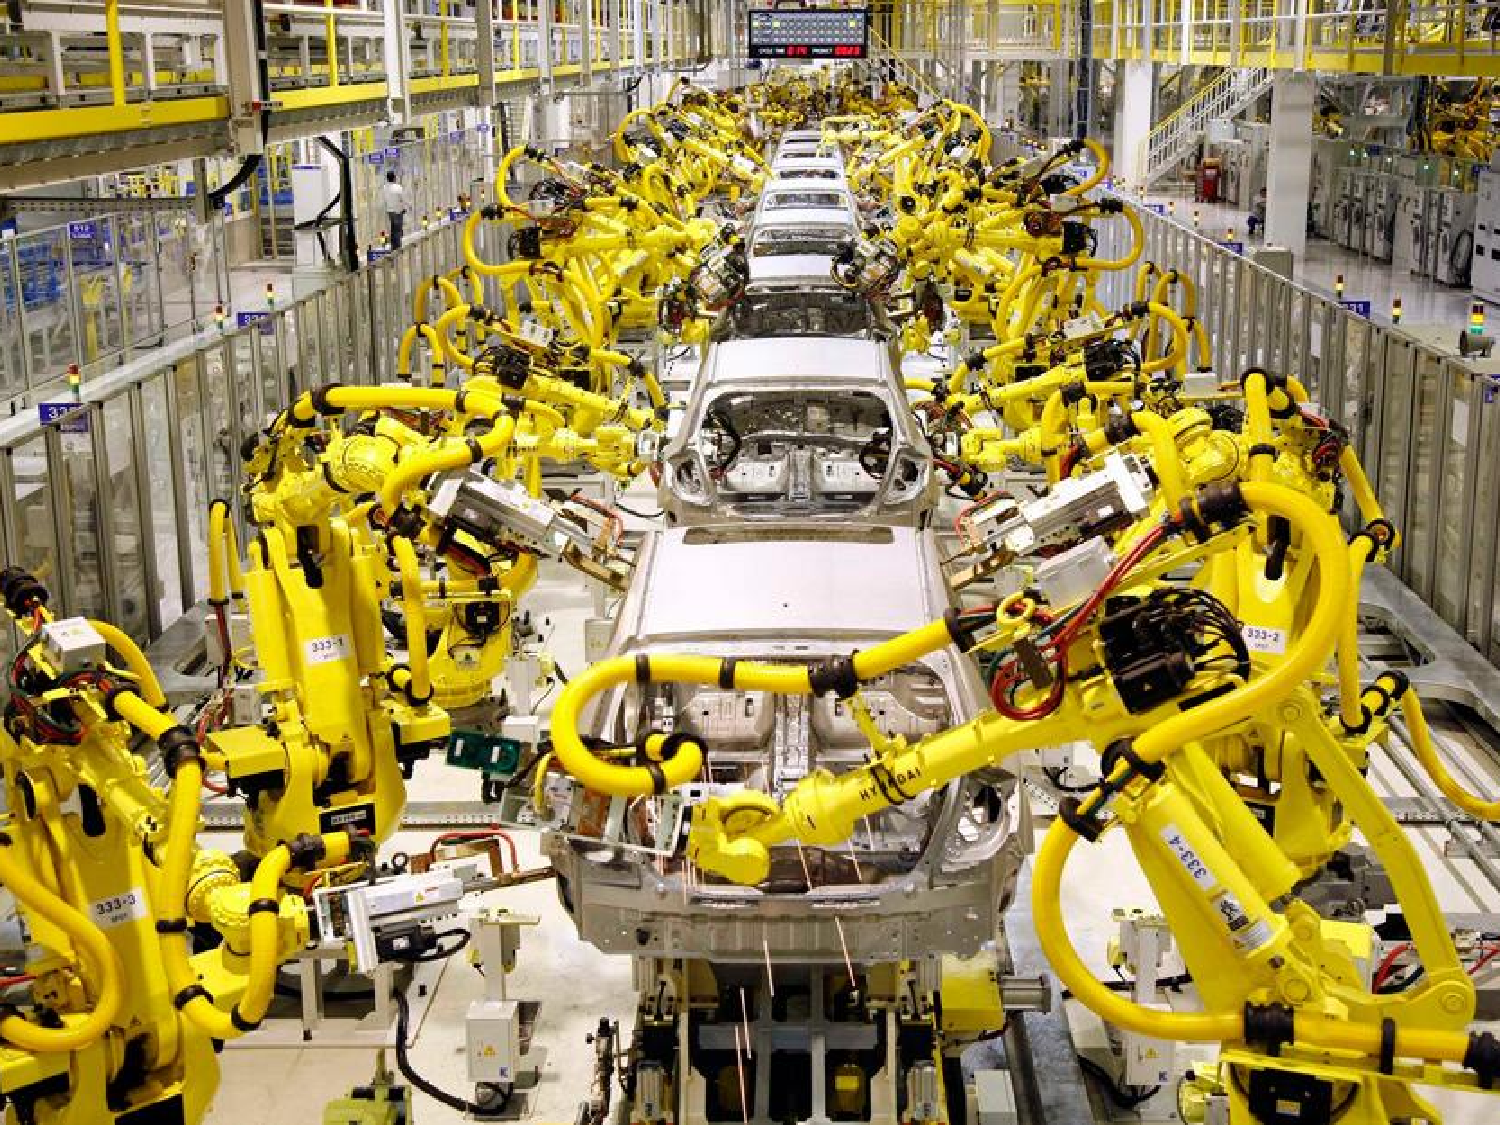
\includegraphics[width=.5\linewidth]{figs/industrial_robot.pdf} \\
        \end{subfigure}
        \\
        \\
        \\
        \\
        %\begin{tabular}{ccc}
        \begin{subfigure}{1.0\linewidth}
            \centering
            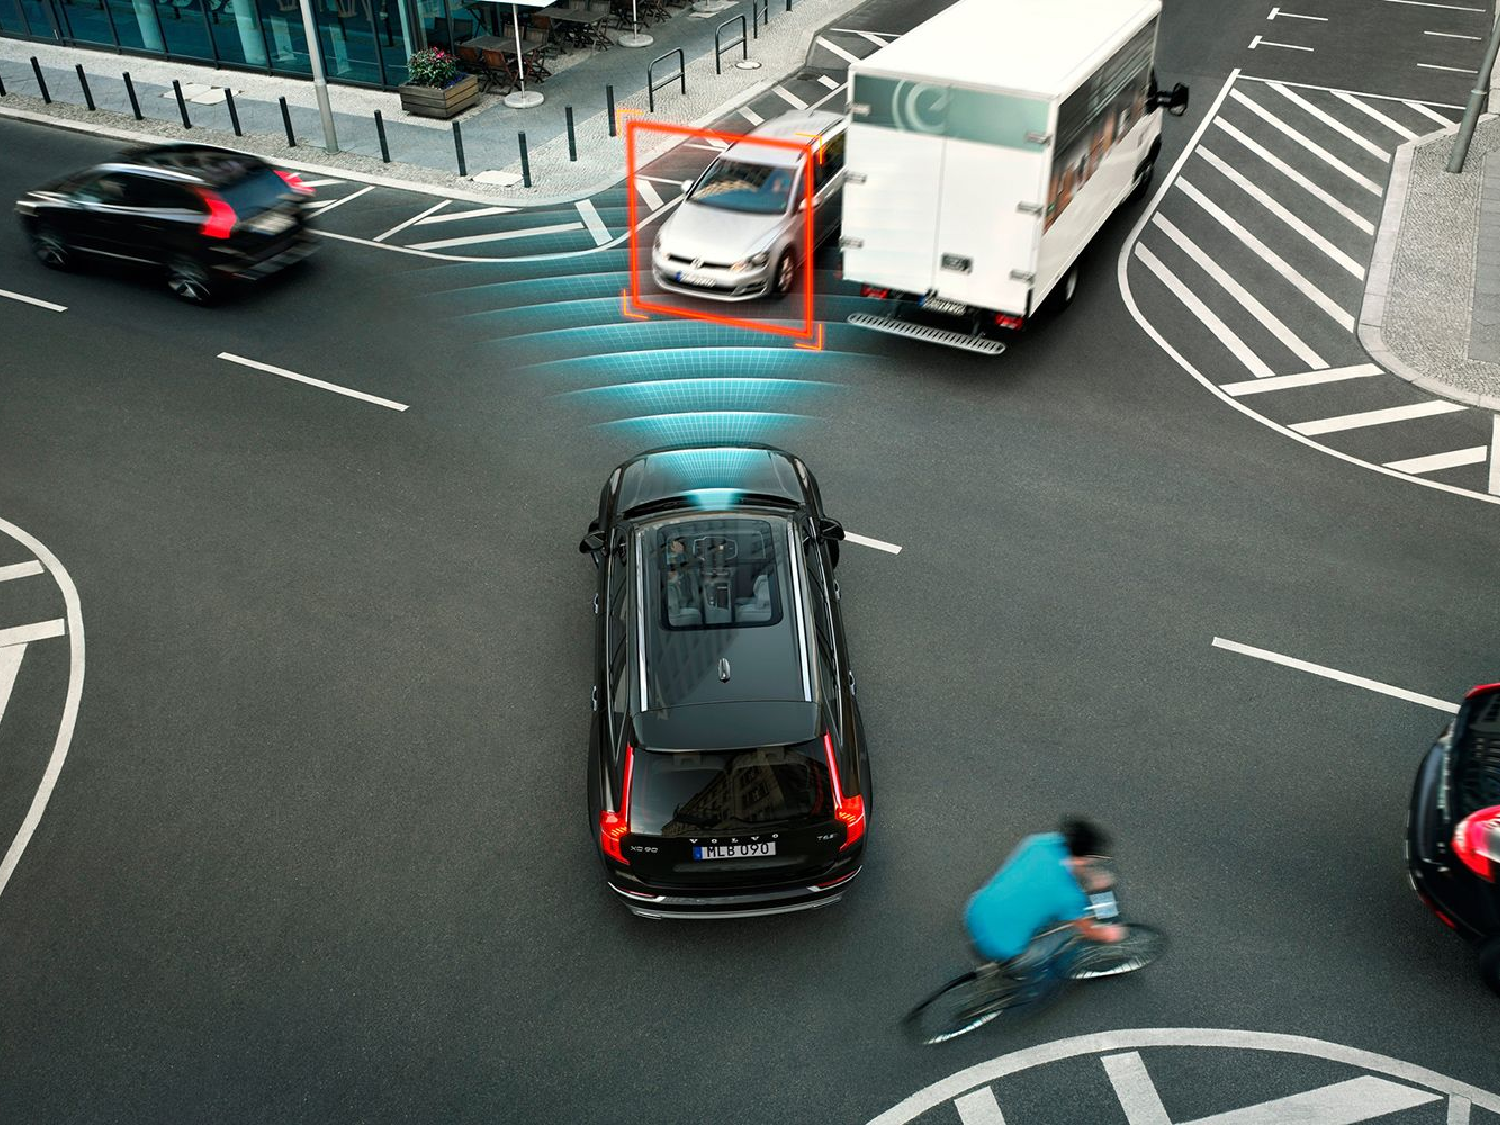
\includegraphics[width=.3\linewidth]{figs/autonomous_car.pdf} 
            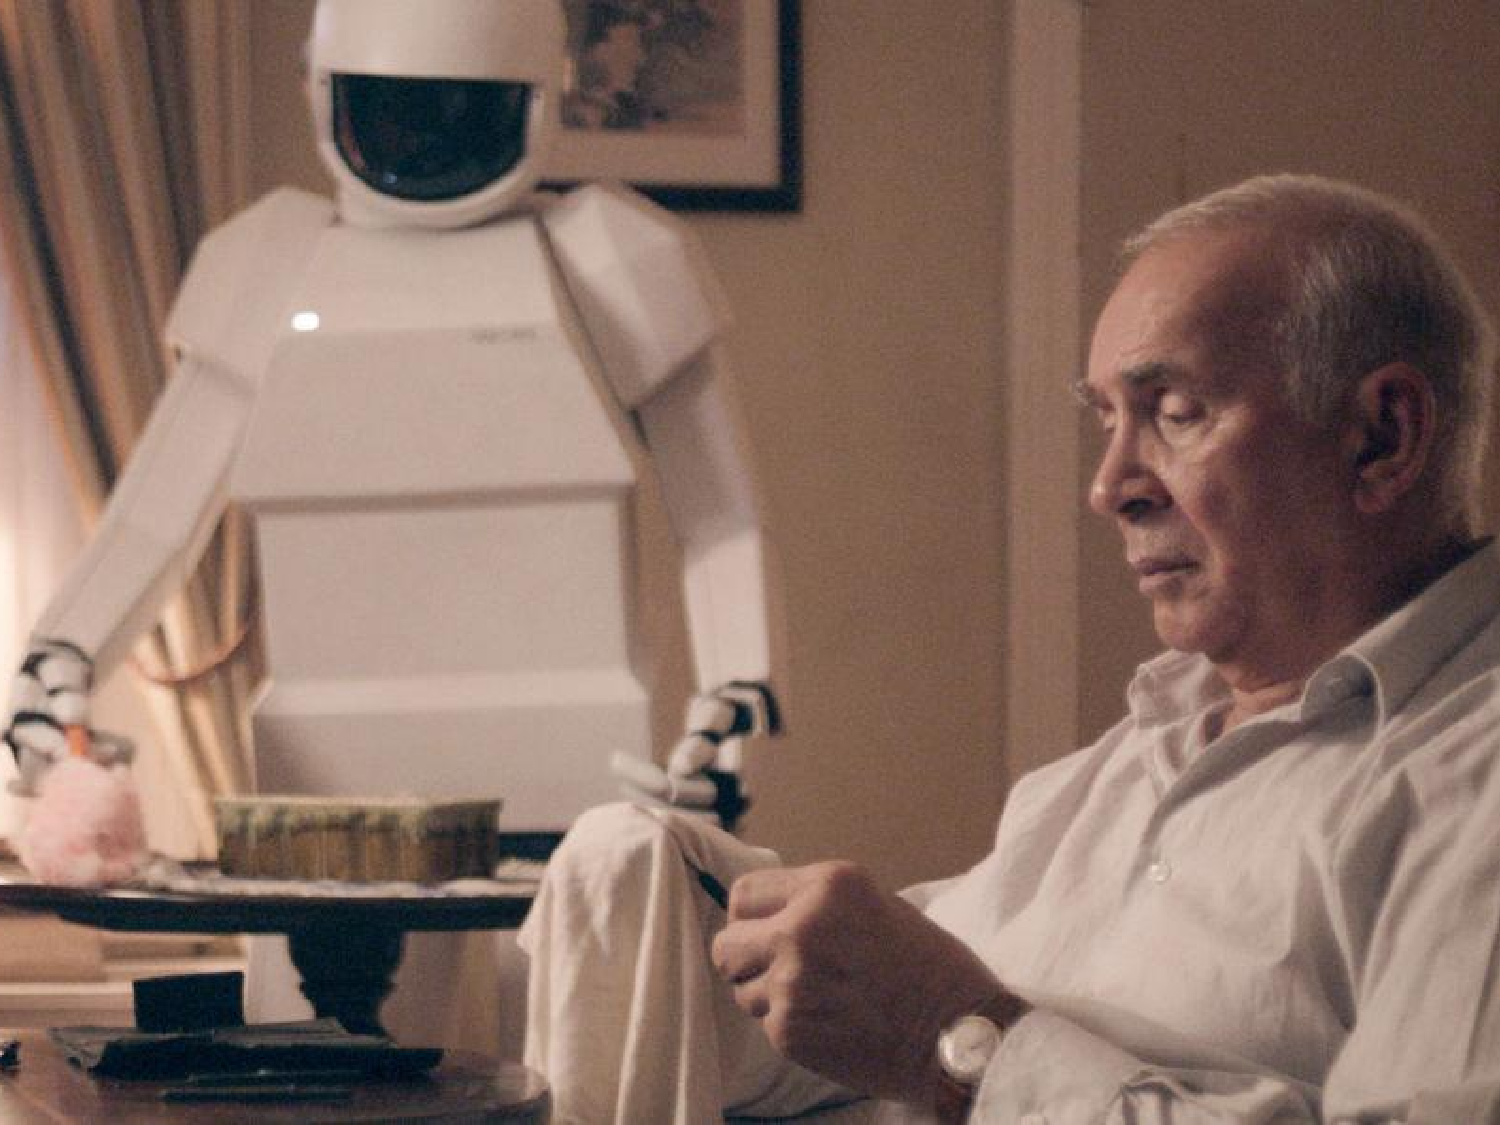
\includegraphics[width=.3\linewidth]{figs/homecare_robot.pdf} 
            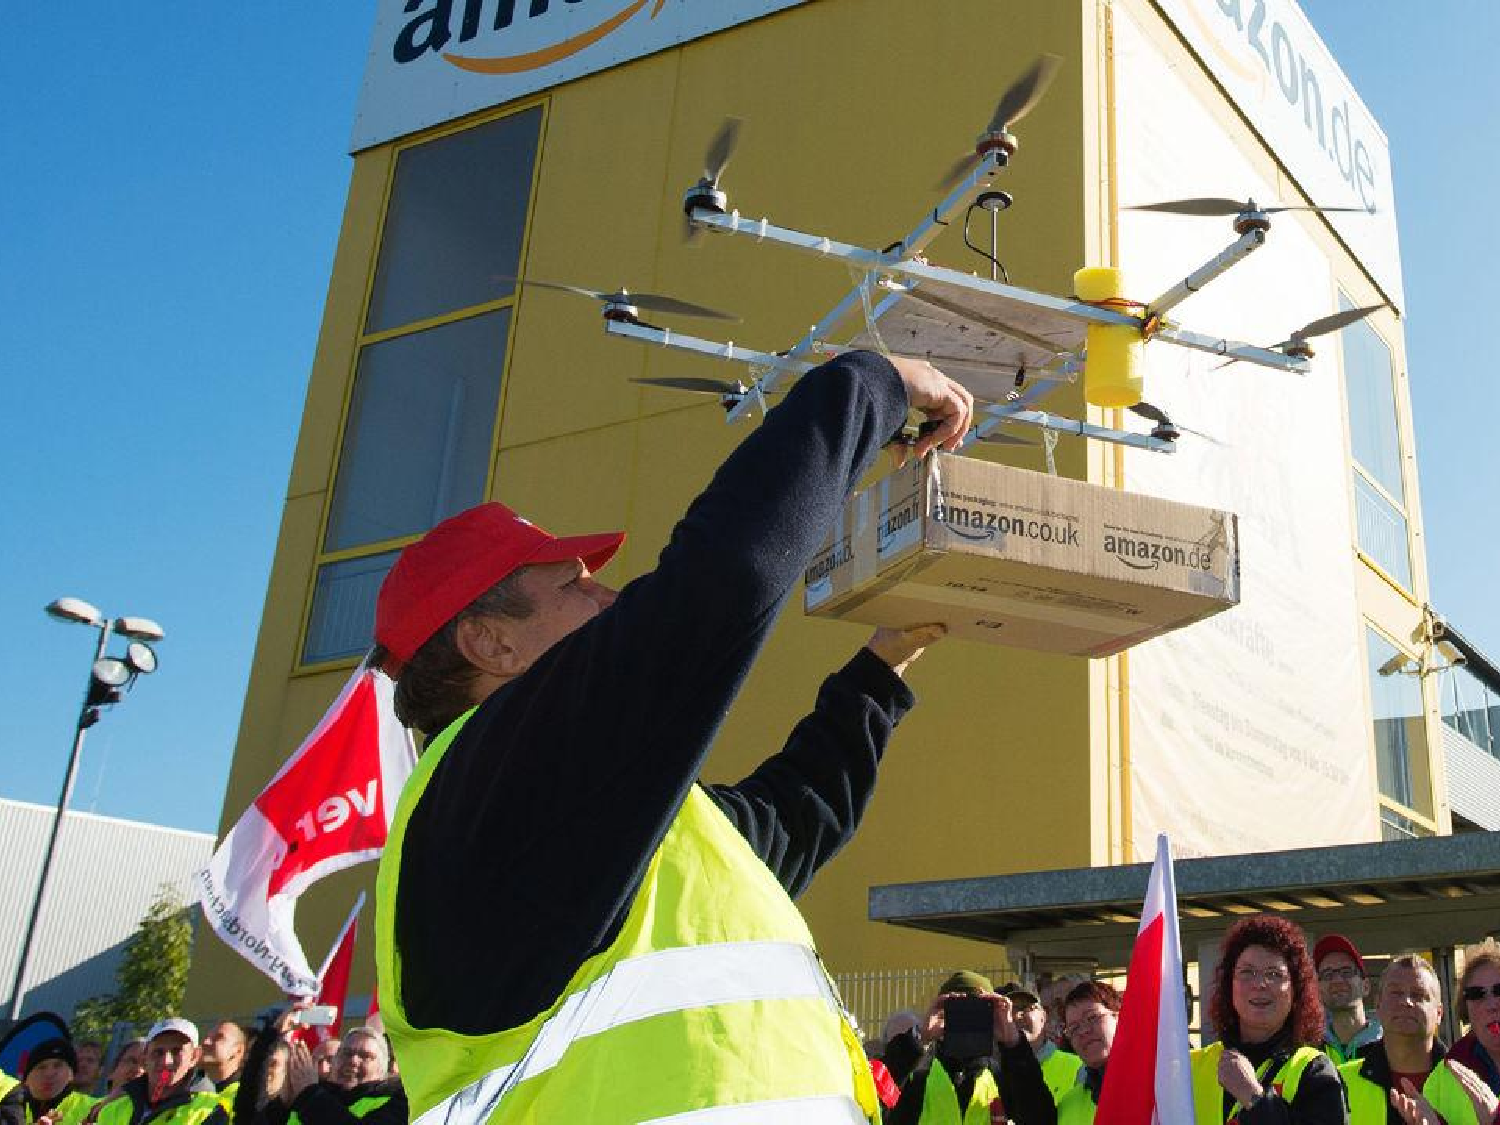
\includegraphics[width=.3\linewidth]{figs/drone_delivery.pdf} 
        \end{subfigure}
    \end{tabular}
    \caption{Top: Robots have their own workspace.
        Bottom: Robots share their workspace with humans.}
    \label{fig:robots}
\end{figure}

% challenges in robot collaborating with humans
Unlike industrial robots,
robot that working closely with human has to 
reason over human's 
physical state and mental state;
and plan its own actions accordingly.

\begin{figure}[!h]
    \centering
    \begin{subfigure}{1.0\linewidth}
        \centering
        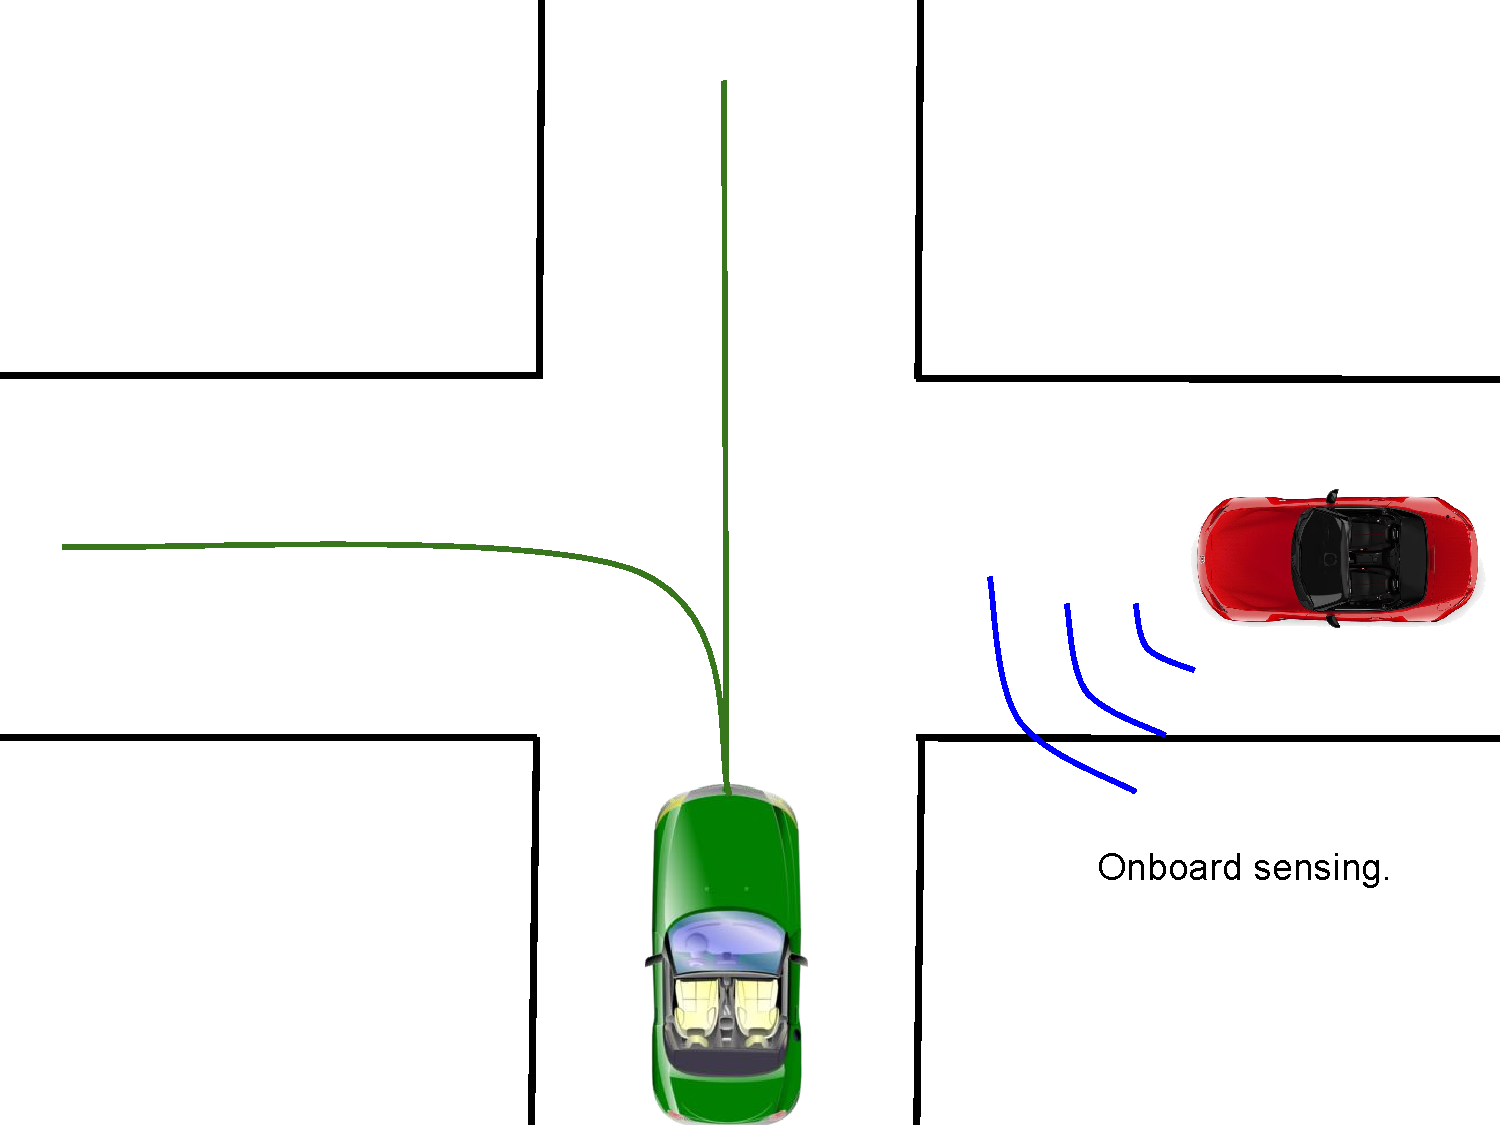
\includegraphics[width=0.4\linewidth]{intersection_nav.pdf}
        \hspace{1.5cm}
        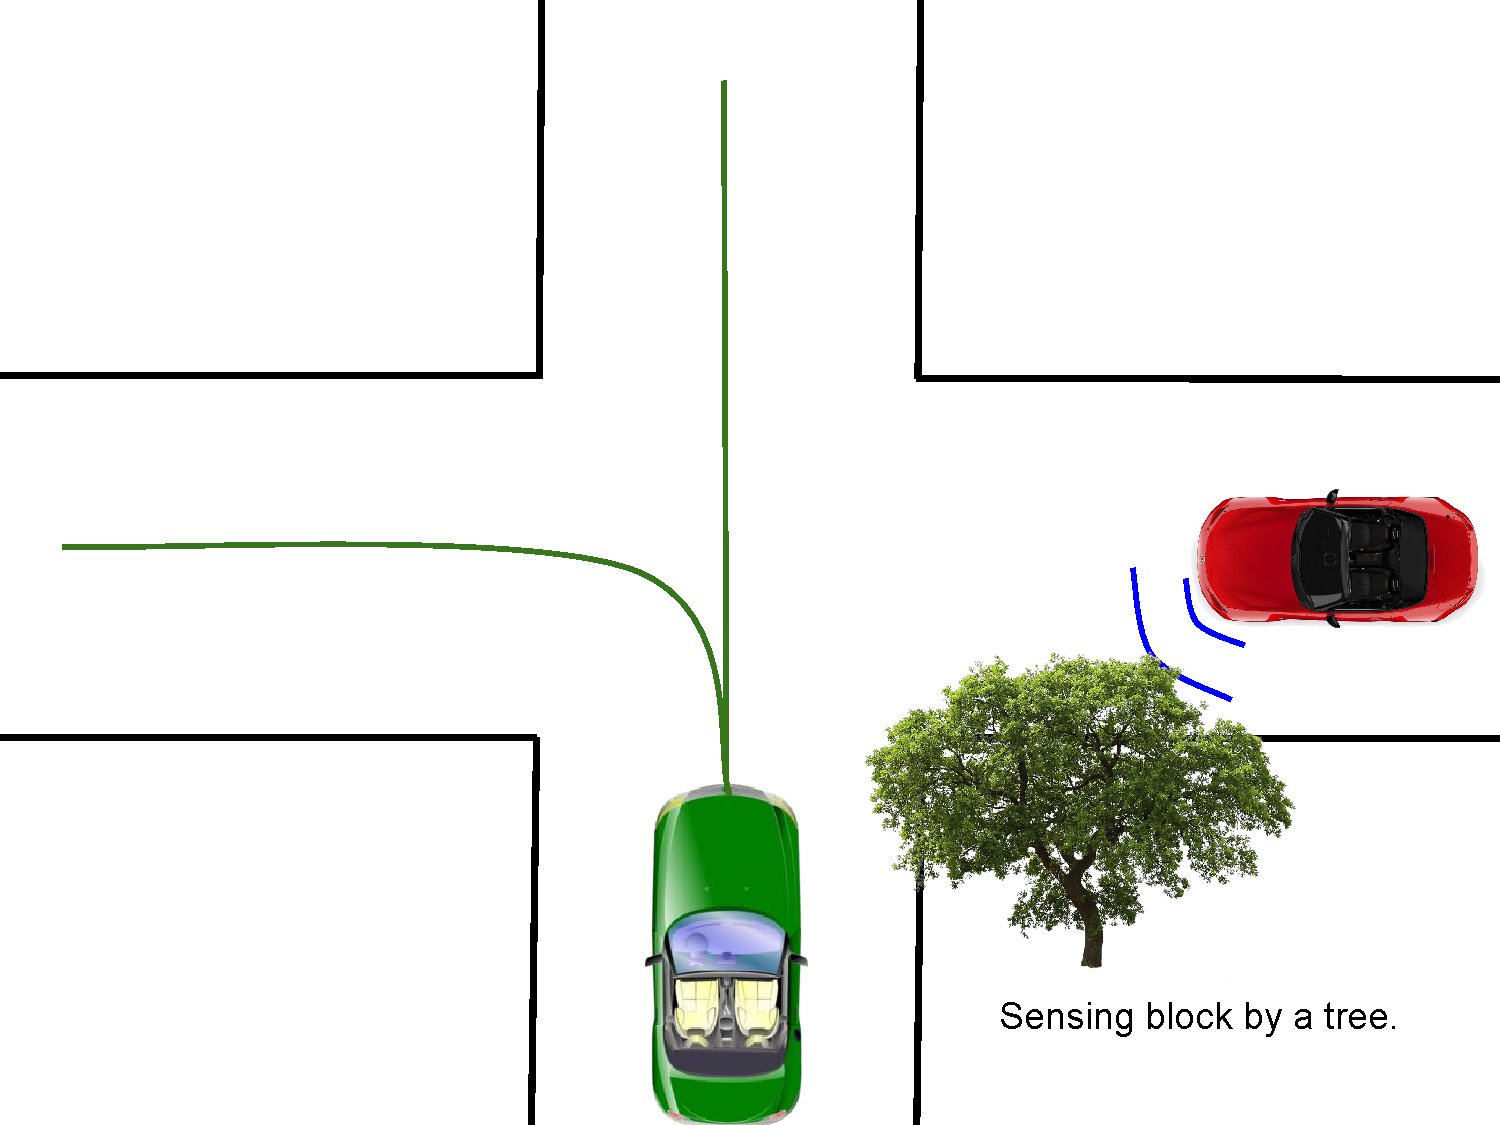
\includegraphics[width=0.4\linewidth]{intersection_nav_block.pdf}
    \end{subfigure}
    \caption{Left column:
        Autonomous car (red) navigating through an unsignalized 
        intersection, with another human driven car (green) around. 
        Right column:
        The onboard sensors might fail due to unexpected obstacles,
        \eg, trees around the road.
    }
    \label{fig:intersection_nav}
\end{figure}


% take an example to explain what is human's mental state, and why it is difficult
Consider an autonomous driving example in~\figref{fig:intersection_nav} (left column).
The autonomous car tries to navigate through an unsignalized intersection
while interacting with another human driver on road. 
Although it is a trival task for human drivers, it
turns out to be extremely difficult for a robot car to perform 
well in such scenario~\cref{cunningham2015mpdm}. 
In order to be safe and efficient, 
the robot car needs to 
know the positions of nearby human driven cars and the paths that 
human drivers are following.


% Current robots rely on onboard sensors
Nowadays, most robots rely purely on onboard sensors,
\eg, lidar and camera \etc,
to gather information from the environment
\cref{siciliano2016springer,thrun2005probabilistic}. 
Onboard sensors provides only limited information for the
robot due to the following reasons.
\begin{itemize}
    \item Onboard can not read humans' mental 
        state, \eg, the sensors will not be able to tell 
        which direction the huma driver is going
        (\figref{fig:intersection_nav}, left column).
    \item Onboard sensors can fail due to unexpected weather
        conditions or obstacles, \eg, the sensors is blocked
        by a tree in the autonomous driving task
        (\figref{fig:intersection_nav}, right column).
\end{itemize}


% Introduce NRC
In this paper, we introduce \nrc, a dApp based 
on NEO blockchain that enables trust-free human-robot 
communication.
With \nrc, (i) the robot can get extra information
by communicate with the human directly, 
\eg, the human can convey his/her intent to the robot 
through the \nrc dApp; 
(ii) the information on the blockchain is guaranteed to
be trustable, and the whole system is more robust to server
failures due to the decentralized nature of blockchain
technology; (iii) the \nrc token provides incentives
for the human to use the dApp and willing the share the
correct information with the robot, \ie, the human will receive
certain amount of tokens as reward once his/her information
is used by a robot and the information is proven to be correct.


% Differentiate NRC from traditional communication devices
Previous works have been working on 
protocols for robot-robot communications 
\cref{yang2004vehicle,torrent2009vehicle,biswas2006vehicle,mclurkin2004distributed}. 
However, none of those protocols can deal with scenarios
when human is in the loop.
Unlike robot-robot communication, human and robot 
have different lauguages and they might not understand
each other. In addition, humans tends to not share their
information with robot for privacy reasons.
\nrc addresses these two issues by providing intuitive
interfaces that are easier for both the human and the robot
to understand, and the \nrc token gives incentives for humans to
share the correct information with the robot.


% Preliminary results on testing NRC on a robot platform
We tested \nrc on the autonomous driving task as a proof of
concept.
(TODO: Preliminary results)


% Impact of NRC
We believe that robots will become more and more popular in
people's daily life, and \nrc provides a general solution
for human-robot information sharing.
Note that, although we demonstrated \nrc on the autonomous
driving task, \nrc is much more general and it can
be potentially applied on any robots that share their workspace
with humans, \eg, service robots in restaurants or hospitals.


\section{Background}
\label{sec:background}

\subsection{Traditional ways of robot information gathering}
\label{subsec:tranditional-ways}

% Onboard sensors


% Robot-robot communication


This part may introduce the current problems faced by robotics in information sharing.

\subsection{Blockchain and smart contracts}
\label{subsec:blockchain}

A blockchain is a decentralized ledger that can record
transactions between two parties in a verfiable and permanent
way without the need for a third authority~\cref{swan2015blockchain}.

Bitcoin is the first public blockchain that serves the purpose
of digital currency~\cref{nakamoto2008bitcoin}.
Few years later, Ethereum launched as the first blockchain with
programmable and Turing complete smart contracts~\cref{wood2014ethereum}.
Smart contracts allows developers to program on the blockchain.
The smart contracts on the blockchain is public that anyone
can inspect, and it will exectued deterministically to achieve
certain goals in a way verifiable to any all involved third
parties.

NEO is China's first publich blockchain, and it is considered to
be a compelling alternative to Ethereum for smart contracts and
distributed applications~\cref{zhang2017neo}.
NEO uses delegated Byzantine Fault Tolerance (dBFT) for 
consensus~\cref{castro1999practical,vukolic2015quest}, 
whereas Ethereum previously used Proof
of Work~\cref{pow2017}, and recently switched to a Proof of Stake
model~\cref{pos2017}.
NEO’s consensus model allows for 
a theoretical transaction throughput up to $10,0000$ tps.
High transaction speed is critical for \nrc, 
since it will most likely require 
real-time communication between many agents.


In addition, NEO supports multiple programming lauguages, such as C\#, Java,
C++, Python, \etc. This makes it easier for developers to develop
smart contract applications on NEO blockchain. 
NEO is rapidly growing its ecosystem with the help from the 
community groups, \eg, City of Zion~\footnote{\url{https://cityofzion.io/}} 
and New Econo Lab~\footnote{\url{https://github.com/NewEconoLab/Docs}}.
We expect to see more and more advanced feature coming out from NEO
platform in the near future.

Considering the various merits of NEO aforementioned, we decide to build
\nrc on NEO blockchain.


\section{NRC for human-robot communication}
\label{sec:nrc}

\subsection{Model}
\label{subsec:model}

\subsection{Prototype}
\label{subsec:prototype}


\section{NRC token}

\subsection{Incentives for humans to share their information 
    with robots}



\subsection{Reward scheme}
What is the reward people can gain by sharing the information.


\section{Proof of concept}
\label{sec:proof-concept}

We can demostrate some interesting examples in this part.

\subsubsection{Robot seeing through the wall}

%\subsubsection{Case Study 2: Avoid the Tesla fatal crash while using autopilot mode}

\section{Roadmap}
\label{sec:roadmap}

We are going to achieve what goals by what time.


%\section*{References}

%References follow the acknowledgments. Use unnumbered first-level
%heading for the references. Any choice of citation style is acceptable
%as long as you are consistent. It is permissible to reduce the font
%size to \verb+small+ (9 point) when listing the references. {\bf
  %Remember that you can go over 8 pages as long as the subsequent ones contain
  %\emph{only} cited references.}

%\medskip

\small

\bibliographystyle{ner-reference-format}
\bibliography{ner}

\end{document}
